\documentclass[UTF8,openany]{ctexbook}

% 论文版面要求:
% 统一按 word 格式A4纸(页面设置按word默认值)编排、打印、制作。
% 正文内容字体为宋体;字号为小4号;字符间距为标准;行距为25磅(约0.88175cm)。

%%%%% ===== 页面设置
\usepackage[a4paper,top=2.54cm,bottom=2.54cm,left=3.17cm,right=3.17cm,%
            ]{geometry}
            
\setlength{\parindent}{2em}
%默认的弹性间距会导致文中某些排版flush的时候,出现大量空白。
\setlength{\parskip}{0.5em} %指定固定段后间距,默认为弹性间距。
\setlength{\intextsep}{10pt} %固定浮浮动体前后间距。


%%%%% =====章节 标题 设置
\ctexset{%
  contentsname={\vspace{-3.5em}\centerline{\zihao{-3}\heiti 目\quad 录}\vspace{-0.7em}},
  listfigurename={\vspace{-3.5em}\centerline{\zihao{-3}\heiti 插\ 图\ 目\ 录}\vspace{-0.5em}},
  listtablename={\vspace{-3.5em}\centerline{\zihao{-3}\heiti 表\ 格\ 目\ 录}\vspace{-0.5em}},
  bibname={\vspace{-3em}\centerline{\zihao{-3}\heiti 参\ 考\ 文\ 献}\vspace{3em}},
  chapter={name={第,章},
           number=\chinese{chapter}, %指定章序号为一二三。。。。
           nameformat={\zihao{3}\bfseries},
           titleformat={\zihao{3}\bfseries},
           beforeskip={-10pt},
           afterskip={20pt}
           },
  section={format=\raggedright,
           nameformat={\zihao{4}\bfseries},
           titleformat={\zihao{4}\bfseries},
%           afterskip={1ex plus 0.2ex}
           beforeskip={1ex},% 固定段前段后间距,
           afterskip={1ex}
           },
  subsection={format=\raggedright,
           nameformat={\zihao{-4}\bfseries},
           titleformat={\zihao{-4}\bfseries},
%           afterskip={0.5ex plus 0.1ex}
           beforeskip={0.5ex},
           afterskip={0.5ex}
           }
}
%%%%% ===== 中英文字体
\setmainfont{Times New Roman}
%\setsansfont{Myriad Pro} % 无衬线字体 sans serif \sffamily
%\setmonofont{Consolas}   % 等宽字体 typewriter \ttfamily
%\newcommand{\Times}{\fontspec{Times New Roman}}
%% 中文字体
%\setCJKmainfont[BoldFont={Microsoft YaHei},ItalicFont={KaiTi}]{NSimSun}
%\setCJKsansfont{Microsoft YaHei}
%\setCJKmonofont{KaiTi}
%\setCJKfamilyfont{STSong}{方正小标宋_GBK}\newcommand{\STSong}{\CJKfamily{STSong}}
\setCJKfamilyfont{songti}{STZhongsong}\newcommand{\STSong}{\CJKfamily{STSong}}

%%%%% ===== 常用宏包
\usepackage{amsmath,amssymb,amsfonts,bm}
\usepackage[amsmath,thref,thmmarks,hyperref]{ntheorem}
\usepackage{graphicx,xcolor,float}
\usepackage{fancyhdr}
\usepackage{tocloft} % 设置目录中的条目间距


\renewcommand\cftdot{\textsubscript{……}}
\renewcommand\cftdotsep{0}

\setlength{\cftbeforechapskip}{1pt}
\renewcommand{\cftchapleader}{\cftdotfill{\cdot}}


\usepackage{booktabs} % toprule, midrule, bottomrule
\usepackage{varwidth} % 可变宽度的 parbox

%%%%% ===== 参考文献与链接
\usepackage[numbers,sort&compress,sectionbib,super, square]{natbib} %引用上标,禁用连续缩写。
\newcommand{\upcite}[1]{\textsuperscript{\cite{#1}}}


\usepackage[xetex,pagebackref]{hyperref}
\hypersetup{CJKbookmarks=true,colorlinks=true,citecolor=blue,%
            linkcolor=blue,urlcolor=blue,bookmarksnumbered=true,%
	        bookmarksopen=true,breaklinks=true}
	        
	        
	        
\iffalse   % 调试时,可去掉,以用于显示引用位置。
\renewcommand*{\backrefalt}[4]{%
\ifcase #1 No citations.%
\or Cited on page #2.%
\else Cited on pages #2.%
%\else #1 Cited on pages #2.%
\fi
}

\else
\renewcommand*{\backrefalt}[4]{}
\fi

%%%%% ===== 浮动图表的标题
\usepackage[margin=2em,labelsep=space,skip=0.5em,font=normalfont]{caption}
\DeclareCaptionFormat{mycaption}{{\heiti\color{blue} #1}#2{\kaishu #3}}
\captionsetup{format=mycaption,tablewithin=chapter,figurewithin=chapter}%,belowskip=-10pt
%\setlength{\belowcaptionskip}{-10pt}

%%%%%% ===== 浮动图表的比例默认50%以下,否则无法浮动。
\renewcommand\floatpagefraction{.9} %当浮动体小于页面90%时进行直接放置。
\renewcommand\topfraction{.9}  
\renewcommand\bottomfraction{.9}  
\renewcommand\textfraction{.1}



%%%%% ===== 算法
\usepackage{algorithm,algpseudocode}

%%%%% ===== 其他
\usepackage{ulem}
\def\ULthickness{1pt}




%%%%%===== Code Style代码
\usepackage{listings}
\usepackage{color}

\definecolor{dkgreen}{rgb}{0,0.6,0}
\definecolor{gray}{rgb}{0.5,0.5,0.5}
\definecolor{mauve}{rgb}{0.58,0,0.82}

\lstset{
  language=Python,
  xleftmargin = 3em,xrightmargin = 3em, aboveskip = 1em,
  aboveskip=3mm,
  belowskip=3mm,
  showstringspaces=false,
  columns=flexible,
  rulesepcolor= \color{gray},
  frame = ltrb,
  basicstyle={\normalsize\ttfamily},
  numbers=none,
  numberstyle=\tiny\color{gray},
  keywordstyle=\color{blue},
  commentstyle=\color{dkgreen},
  stringstyle=\color{mauve},
  breaklines=true,
  breakatwhitespace=true,
  tabsize=3
}


\newcommand{\mcc}[1]{\multicolumn{1}{c}{\underline{\makebox[10em][c]{#1}}}}
\newcommand{\mce}[1]{\multicolumn{1}{c}{\underline{\makebox[15em][l]{#1}}}}


\pagestyle{fancy}
\fancyhf{}  % 清除以前对页眉页脚的设置

\newcommand{\makeheadrule}{%% 定义页眉与正文间双隔线
    \makebox[0pt][l]{\rule[.7\baselineskip]{\headwidth}{0.3pt}}%0.4
    \rule[0.85\baselineskip]{\headwidth}{1.0pt}\vskip-.8\baselineskip}
\makeatletter
\renewcommand{\headrule}{%
    % {\if@fancyplain\let\headrulewidth\plainheadrulewidth\fi\makeheadrule}}
    {\makeheadrule}}
\makeatother
\renewcommand{\chaptermark}[1]{\markboth{\CTEXthechapter \ #1}{}}
\renewcommand{\sectionmark}[1]{\markright{\thesection \ #1}{}}
%\fancyhead[RO,LE]{{\small\songti\rightmark}}     % 节标题
%\fancyhead[RE]{{\small\songti\leftmark}}      % 章标题
\fancyhead[L]{《人工智能的数学思维》课程报告}
\fancyhead[R]{矩阵运算与网页排名}
% \fancyhead[RO,LE]{$\cdot$ {\small\thepage} $\cdot$}
\fancyfoot[C]{{-\thepage-}}
%\fancyfoot[CO,CE]{{\thepage}}



\begin{document}

\begin{titlepage}
    \begin{center}
        \begin{figure}[H]
            \vspace{5cm}
            
\includegraphics[width=14cm]{images/ecnu.png}
        \end{figure}
        {
        \heiti\zihao{2}《人工智能的数学思维》课程报告\\
        \vspace{0.8em}
        \songti\zihao{1}\textbf{矩阵运算与网页排名}
        }
        \\[10em]
        \zihao{-3}
        \begin{tabular}{p{0cm}p{5.5em}@{\extracolsep{0.5ex}}cc}
            ~ & \hfill 组 \quad 员: &  & \mcc{李鹏达 10225101460} \\
            ~ & \hfill               &  & \mcc{武泽恺 10225101429}   \\
            ~ & \hfill               &  & \mcc{吴泽霖 10225101428}   \\
            ~ & \hfill               &  & \mcc{张耘彪 10225101437}   \\
        \end{tabular}
        \\[8em]
        \zihao{-2}2023年4月
    \end{center}
    \thispagestyle{fancy}
    \fancyfoot[C]{}
\end{titlepage}
\fancyfoot[C]{-\thepage-}
% \clearpage%{\pagestyle{empty}\cleardoublepage}
\pagestyle{fancy}
\phantomsection

\centerline{\zihao{-3}\heiti \textbf{摘\quad 要}}
\addcontentsline{toc}{chapter}{摘\quad 要}

\linespread{1.1}\zihao{-4} \bigskip
\kaishu
矩阵运算和线性代数是计算机科学中非常重要的数学概念,Google作为全球最大的搜索引擎,其使用的PageRank算法是一种基于矩阵运算的著名算法。PageRank算法是谷歌搜索引擎中用来对网页进行排序的算法之一,该算法通过分析网页之间的链接关系来确定网页的重要性。

在PageRank算法中,每个网页被视为矩阵中的一个节点。通过矩阵运算,算法可以计算每个网页的PageRank值,从而确定网页的重要性。

本文将介绍PageRank算法的原理及其与矩阵运算的关系。我们将探讨如何使用矩阵运算来计算PageRank值,并讨论该算法在人工智能中的应用。
\bigskip

\noindent{\zihao{4}\heiti 关键词:}
PageRank,网页排名,矩阵运算,搜索引擎
\songti
\setcounter{page}{1}
\pagenumbering{roman}

\newpage

\tableofcontents
\thispagestyle{fancy}
\addcontentsline{toc}{chapter}{目\quad 录}

\newpage

\listoffigures
\thispagestyle{fancy}
\addcontentsline{toc}{chapter}{插图目录}

\newpage
\pagenumbering{arabic}
\setcounter{page}{1}
\chapter[引言]{引言}
\thispagestyle{fancy}
\section[前言]{前言}
Google作为世界上最大的搜索引擎,在市场上占有巨大的份额。
如图1.1所示,网站Statcounter GlobalStats的数据显示\cite{bi:SG},2023年3月,在全球范围的统计下,Google占据了搜索引擎份额的$93.18\%$。而它的竞争对手们——bing占据了$2.87\%$,Yahoo为$1.12\%$,YANDEX为$1.02\%$,DuckDuckGo为$0.52\%$,百度为$0.42\%$。可以说,Google在搜索引擎业务上几乎占据了绝对的垄断地位。
\begin{figure}[H]
    \begin{center}
        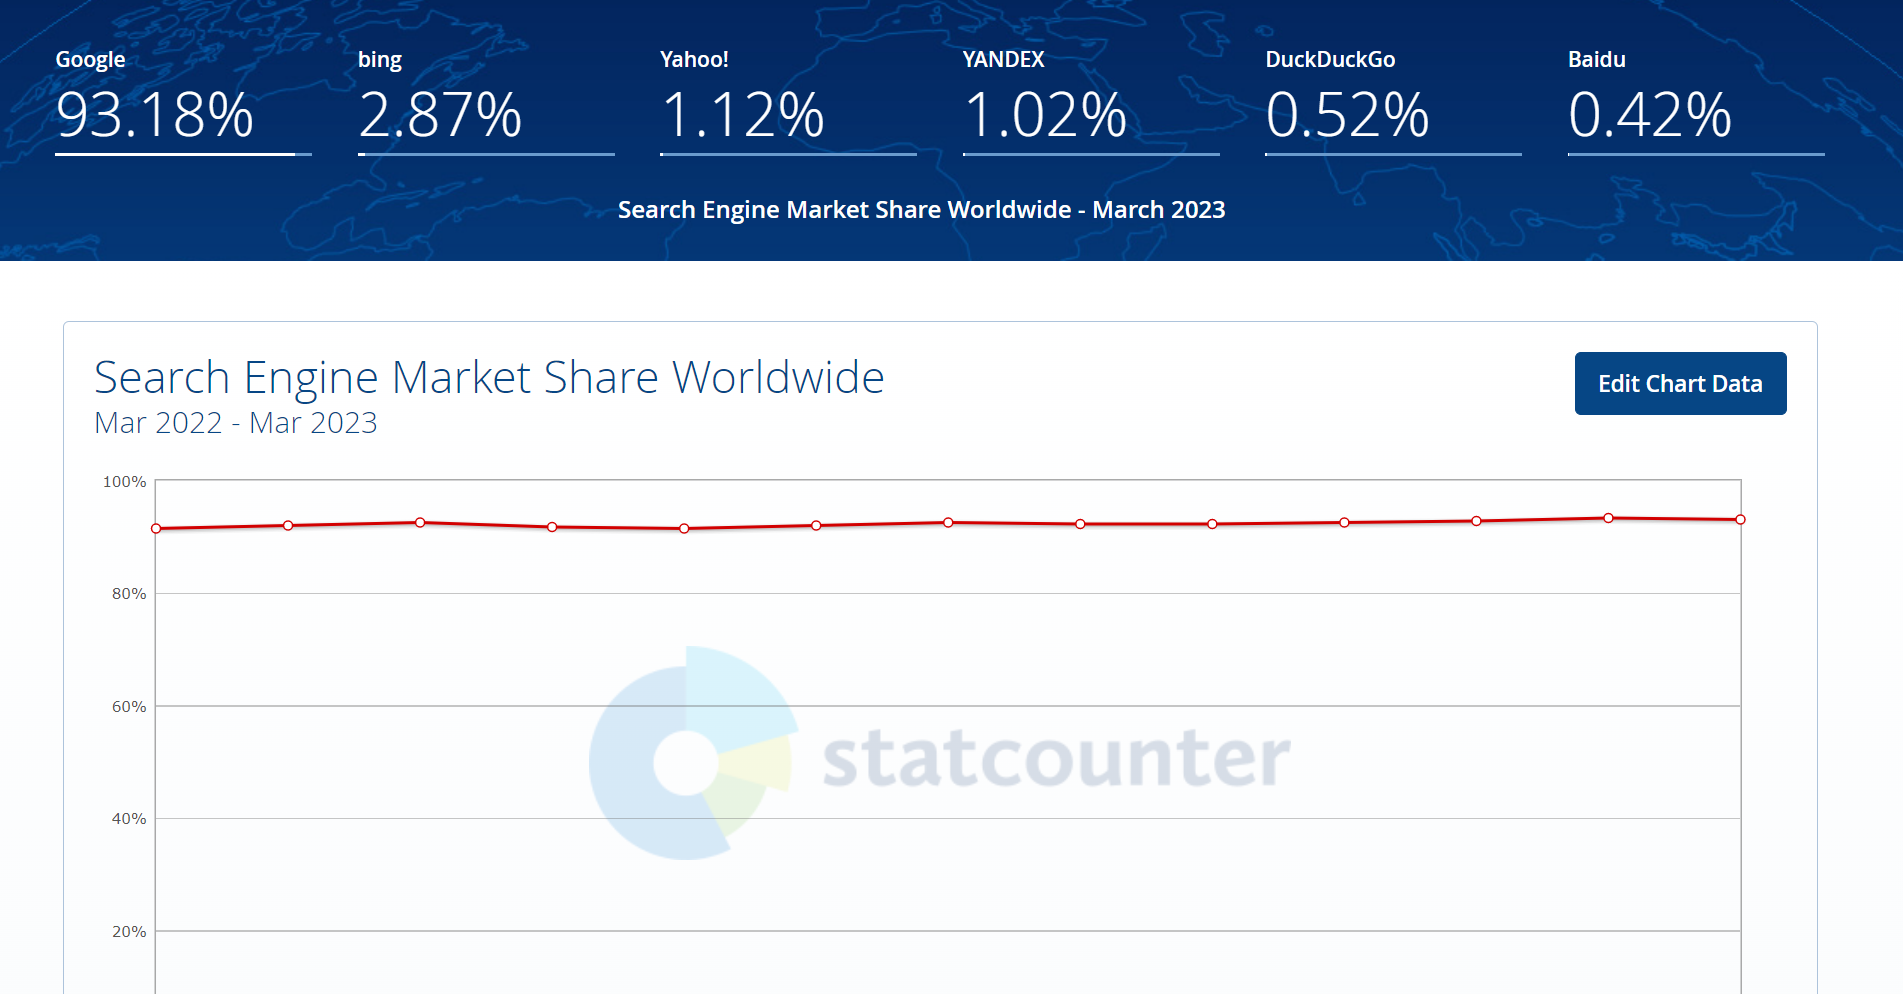
\includegraphics[width=0.9\textwidth]{images/statcounter.png}
        \caption{Statcounter GlobalStats统计的2023年3月全球市场搜索引擎份额}
    \end{center}
\end{figure}

而Google的垄断地位离不开其强大的检索功能和高质量的检索服务。

例如,我们在Google上搜索“大夏学堂”,得到的结果如图1.2所示,排名第一的是华东师范大学大夏学堂官网,排名第二的是ECNU Forum上关于大夏学堂相关问题的提问,排名第三的是华东师范大学课程中心关于大夏学堂停机升级的公告,接下来的则是大夏学堂优质示范课程。

而当我们在某其他搜索引擎上搜索“大夏学堂”时(如图1.3所示),虽然排在首位的仍是华东师范大学大夏学堂官网,排名第二的却是某小说网站上与小说《大夏学堂》有关的内容。这明显不是我们想要得到的搜索结果。

这是一个值得探究的问题。Google是如何对搜索得到的结果进行排序,从而保障用户期望的搜索结果,即较为“重要”的网站排名靠前,而“不重要”或与搜索内容关联较小的网站排在后方?

这主要依赖排序机制。排序机制是Google保证搜索质量的关键。其主要依靠PageRank算法,该算法可以判断网页的重要性和权威度,决定其在搜索结果中的排名。Google精准而高效的搜索结果排序,与其 PageRank算法和对用户的深刻理解是密不可分的。这是Google持续领先于同业的核心因素之一,也是接下来我们要重点介绍的内容。

\begin{figure}[H]
    \begin{center}
        \begin{minipage}[b]{0.49\textwidth}
            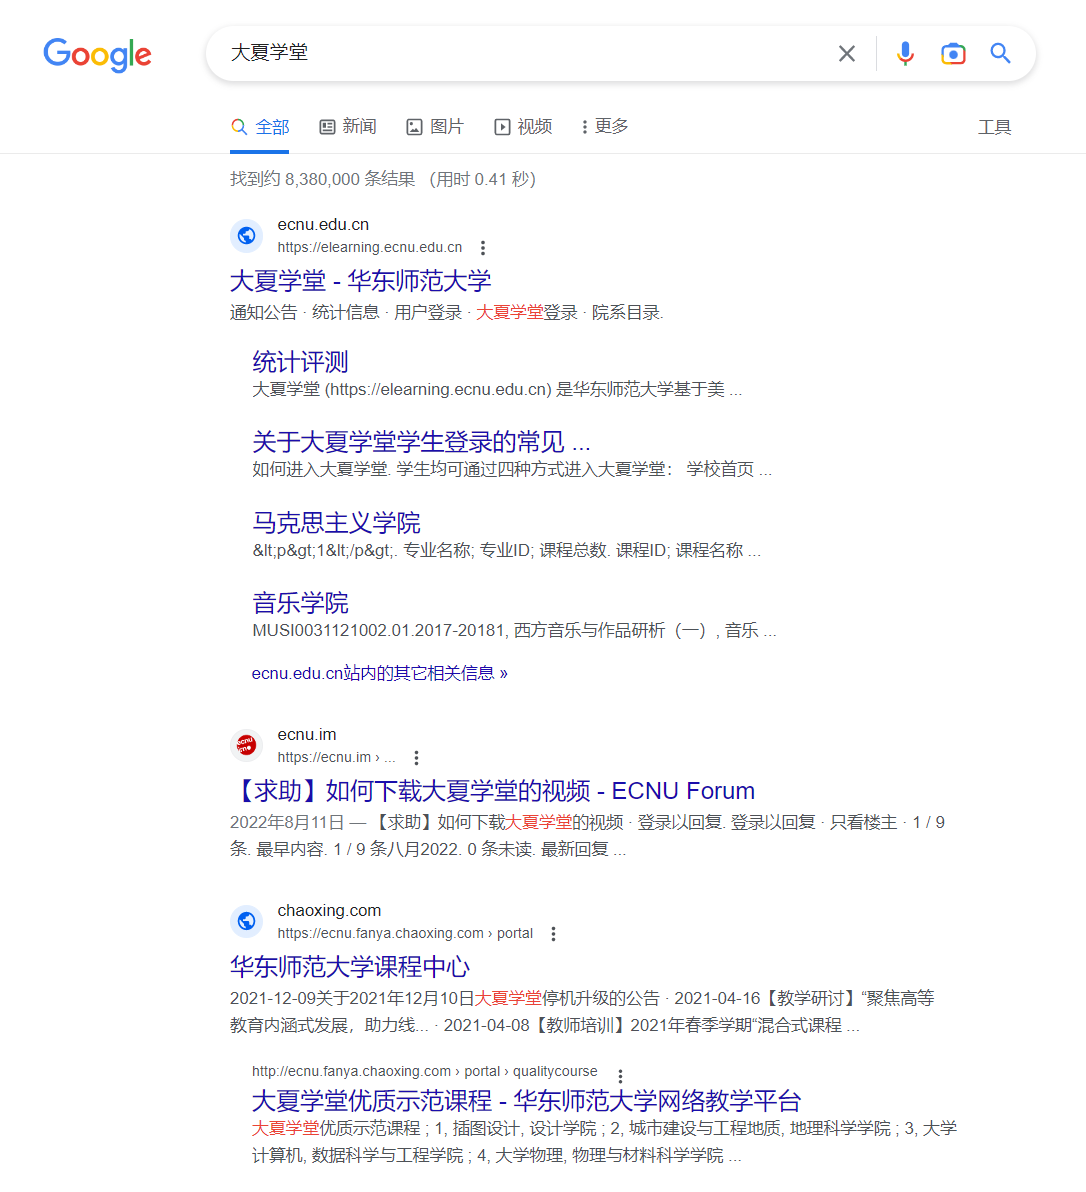
\includegraphics[width=0.9\textwidth]{images/daxia_google.png}
            \caption{在Google上搜索“大夏学堂”得到的结果}
        \end{minipage}
        \begin{minipage}[b]{0.49\textwidth}
            
\includegraphics[width=0.9\textwidth]{images/daxia_baidu.png}
            \caption{在某搜索引擎上搜索“大夏学堂”得到的结果}
        \end{minipage}
    \end{center}
\end{figure}

\section[涉及到的概念与方法]{涉及到的概念与方法}
\subsection[PageRank简介]{PageRank简介}
PageRank,又称网页排名、PR,是Google公司所使用的对其搜索引擎搜索结果中的网页进行排名的一种算法。

PageRank本质上是一种以网页之间的超链接个数和质量作为主要因素粗略地分析网页的重要性的算法。其基本假设是:更重要的页面往往更多地被其他页面引用(或称其他页面中会更多地加入通向该页面的超链接)。 其将从A页面到B页面的链接解释为“A页面给B页面投票”,并根据投票来源(甚至来源的来源,即链接到A页面的页面)和投票对象的等级来决定被投票页面的等级。简单的说,一个高等级的页面可以提升其他低等级的页面。

\begin{figure}[H]
    \begin{center}
        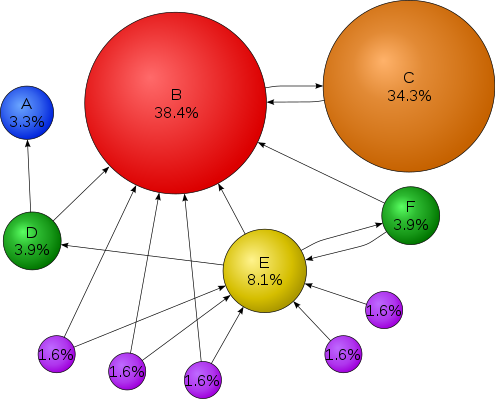
\includegraphics[width=0.6\textwidth]{images/PageRanks-Example.svg.png}
        \caption{PageRank算法的一个简单示例}
    \end{center}
\end{figure}

该算法以谷歌公司创始人之一的拉里·佩奇(Larry Page)的名字来命名。谷歌搜索引擎用它来分析网页的相关性和重要性,在搜索引擎优化中经常被用来作为评估网页优化的成效因素之一。

目前,PageRank算法不再是谷歌公司用来给网页进行排名的唯一算法,但它是最早的,也是最著名的算法。



\subsection[马尔可夫链简介]{马尔可夫链简介}
马尔可夫链(Markov chain),又称离散时间马尔可夫链,因俄国数学家安德烈·马尔可夫得名,为状态空间中经过从一个状态到另一个状态的转换的随机过程。该过程要求具备“无记忆”的性质:下一状态的概率分布只能由当前状态决定,在时间序列中它前面的事件均与之无关。这种特定类型的“无记忆性”称作马尔可夫性质。马尔科夫链作为实际过程的统计模型具有许多应用。

在马尔可夫链的每一步,系统根据概率分布,可以从一个状态变到另一个状态,也可以保持当前状态。状态的改变叫做转移,与不同的状态改变相关的概率叫做转移概率。

当马尔可夫链运行足够长时间后,无论初始状态是什么,其状态的概率分布会达到平稳分布,并且保持不变。
形式上,如果马尔可夫链有$n$个状态,转移矩阵为$P$,平稳分布向量为$\boldsymbol{\pi}$,则需要满足$\boldsymbol{\pi} = \boldsymbol{\pi} P$。


这表示平稳分布向量$\boldsymbol{\pi}$是转移矩阵$P$的特征向量,对应特征值为$1$。
具体来说,平稳分布具有以下性质:

\begin{enumerate}
    \item $\boldsymbol{\pi}_i \ge 0$,且$\sum\boldsymbol{\pi}_i = 1$。即平稳分布的每个元素都非负,且和为$1$,代表概率。
    \item $\boldsymbol{\pi}=\boldsymbol\pi P$。即平稳分布向量是转移矩阵的特征向量,对应特征值为$1$。这说明如果当前状态按平稳分布,那么过一步转移后,状态的分布仍然是平稳分布。
    \item 不依赖初始状态。无论初始状态是什么,经过足够长时间转移,马尔可夫链的状态分布会达到平稳分布。
    \item 唯一性。马尔可夫链的平稳分布是唯一的。
\end{enumerate}

平稳分布表示马尔可夫链在长期运行后的稳定态,不会再被初始状态影响。它衡量了每个状态在整个链中出现的频率,给出了马尔可夫链稳定运行时每个状态上花费的时间比例。

假设我们在上网浏览页面时,选择下一个界面的过程,与过去浏览过哪些界面没有关系,而仅依赖于当前的页面。这是一个简单的有限状态、离散时间的随机过程,可以使用马尔可夫链来描述。

\section[本报告的主要结构和内容]{本报告的主要结构和内容}
本报告分为六章,将主要介绍PageRank网页排名算法的背景、详细内容、应用、缺陷和优化,并简单介绍其在人工智能领域的应用。

同时,本报告将重点分析线性代数(尤其是矩阵运算)以及其他数学思维在PageRank算法中发挥的作用,并给出具体的PageRank计算实例。


\chapter[PageRank算法的详细介绍]{PageRank算法的详细介绍}
\thispagestyle{fancy}
\section[背景]{背景}
PageRank算法与矩阵的特征值有关。在PageRank算法被提出之前,特征值问题就在许多评分问题中被重用。许多人独立地提出使用特征值问题,包括Edmund Landau在1895年关于决定国际象棋锦标赛获胜者的建议、Gabriel Pinski和Francis Narin在1976年关于科学计量学排名科学期刊的工作、Thomas Saaty在1977年提出的层次分析过程概念中加权替代选择、以及Bradley Love和Steven Sloman在1995年作为概念的认知模型,即中心性算法。此外,Robin Li于1996年开发的RankDex搜索引擎使用了类似PageRank的策略来评分和排名网站。

Google的创始人Larry Page和Sergey Brin于1996年在斯坦福大学开发了PageRank算法作为一项新型搜索引擎的研究项目的一部分。他们以PageRank为基础创建了Google搜索引擎,而PageRank算法依然是Google搜索工具的基础之一。

\section[基本原理]{基本原理}

PageRank算法的基本原理与矩阵运算有关。

首先,假设互联网上共有$n$个页面,可以按照如下方式定义一个$n \times n$的超链接矩阵$P$。假设页面$i$拥有$k>0$个指向其他页面的超链接,则如果$i$和$j$之间有这样的一条超链接,$P_{ij}=1/k$,否则$P_{ij}=0$,即
\begin{equation}
    P_{ij}=\begin{cases}
        1/k, & \text{存在由$i$指向$j$的超链接} \\
        0,   & \text{其他情况}
    \end{cases}
\end{equation}

为了使此超链接图联通,可以假设浏览者以一定的概率访问均匀分布的任意网页。因此,可以将其定义为马尔可夫链的平稳分布,其状态空间为所有网页的集合,转移矩阵为
\begin{equation}
    \widetilde{P}=cP+\frac{(1-c)}{n}E
\end{equation}
其中,$E$是一个元素全为$1$的矩阵,$n$是网页页面的数量,$c \in (0,1)$是模型参数,我们将其称为“阻尼因子”,它表示用户不会终止当前界面的浏览且随机跳转到任意界面的概率,通常取0.85\cite{bi:G}。

由于矩阵$\widetilde{P}$是随机矩阵,非周期性且不可约,根据马尔科夫链的理论\cite{bi:RA},存在唯一的平稳分布向量$\boldsymbol{\pi}$,使得它是转移矩阵$\widetilde{P}$的特征向量,对应特征值是$1$\cite{bi:DGPOLS}。即
\begin{equation}
    \boldsymbol{\pi} \widetilde{P}=\boldsymbol{\pi},\quad\boldsymbol{\pi}\boldsymbol{e}=1
\end{equation}
其中,$\boldsymbol{e}$为元素全为1的列向量。

我们将满足式(2.3)的向量$\boldsymbol{\pi}$称为PageRank向量,如果一个浏览者以概率$c$跟随网页上的一个超链接,而以概率$(1-c)$跳转到一个随机界面,那么$\boldsymbol{\pi_i}$可以被解释为该浏览者在页面$i$的平稳概率。

最终,得到的PageRank向量的各分量即为各网页的PageRank值。

实际上,每次计算得到的PageRank值也可以用另一个公式
\begin{equation}
    PR(A)=\frac{1-c}{n} + c\sum_i \frac{PR(T_i)}{L(T_i)}
\end{equation}
来描述。
其中,$A$为所求节点,$PR(T_i)$为其他节点(存在指向$A$的超链接的节点)的PageRank值,$L(T_i)$为其他节点的指向其他页面的超链接数(即式(2.1)中的$k$值)。不难发现,公式(2.2)和(2.3)为公式(2.4)的矩阵表示。


\section[计算方法]{计算方法}

PageRank 可以通过迭代法或代数法计算。迭代法可以视为幂迭代法或幂方法。两种方法执行的基本数学运算是相同的。代数法是通过构建并解决一个描述网页关系的线性方程组来计算PageRank值的。这需要构造一个非常大的矩阵,并且解方程组也很困难,计算复杂度高。迭代法顾名思义就是通过重复迭代逼近最终解。它的基本思想是:每个网页的PageRank值都等于其他所有指向它的网页的PageRank值之和除以对应网页的出链总数。通过多次迭代计算,PageRank值会逐步收敛至稳定。

因此,在本部分,我们仅介绍迭代法。

\subsection[迭代原理]{迭代原理}

我们使用$PR(x,i)$来表示页面$x$在第$i$次迭代时得到的PageRank值。在$i=0$时,我们需要对各网页的PageRank值进行初始化,通常取
\begin{equation}
    PR(P_i,0)=\frac{1}{n}
\end{equation}
接下来,根据公式(2.4),我们对PageRank值进行迭代计算
\begin{equation}
    PR(P_i,i+1)=\frac{1-c}{n} + c\sum_i \frac{PR(P_j, i)}{L(P_i)}
\end{equation}
或根据公式(2.2)和(2.3)使用矩阵表示
\begin{equation}
    \boldsymbol{\pi}_{i+1}=\boldsymbol{\pi}_i\widetilde{P}=cP\boldsymbol{\pi}_i+\frac{1-c}{n}\boldsymbol{e}
\end{equation}
根据公式(2.6)或公式(2.7)我们可以通过重复迭代计算至其收敛,满足
\begin{equation}
    |PR(P_i, i+1)-PR(P_i, i)|<\epsilon
\end{equation}
其中,$\epsilon$是一个很小的值。此时的PageRank值即可视为网页的最终PageRank值。

\subsection[幂迭代法]{幂迭代法}
设超链接矩阵为$P$,向量$\boldsymbol{\pi}$为平稳分布向量(即其满足公式(2.3)),则有
\begin{equation}
    \boldsymbol{\pi}=(cP+\frac{1-c}{n}E)\boldsymbol{\pi}=\widetilde{P}\boldsymbol{\pi}
\end{equation}
故$\boldsymbol{\pi}$为矩阵$\widetilde{P}$的特征向量。

因此,便存在一种快速简便的计算方法——幂迭代法:从任意向量$\boldsymbol{x}(0)$开始,不断地与矩阵$\widetilde{P}$进行运算
\begin{equation}
    \boldsymbol{x}(t+1)=\widetilde{P}\boldsymbol{x}(t)
\end{equation}
直至
\begin{equation}
    |\boldsymbol{x}(t+1)-\boldsymbol{x}(t)|<\epsilon
\end{equation}
此时,向量$\boldsymbol{x}(t)$即为PageRank向量$\boldsymbol{\pi}$。

\subsection[代码实现]{代码实现}
可以使用Python实现上述幂迭代法。

\begin{lstlisting}
  import numpy as np
  def pagerank(P: np.array, num: int = 100, c: float = 0.85):
      P = np.transpose(P)
      N = P.shape[1]
      v = np.ones(N) / N
      P_hat = c * P + (1 - c) / N
      for _ in range(num):
          v = P_hat @ v
      return v
\end{lstlisting}
其中,参数$P$为超链接矩阵$P$,参数$num$为迭代次数,参数$d$为阻尼系数$d$。

\chapter[简单的PageRank实例]{简单的PageRank实例}

\section[实例1:影响PageRank的因素]{实例1:影响PageRank的因素}
考虑一个仅由四个网页组成的简单网络,结构如下图所示。
\begin{figure}[H]
    \begin{center}
        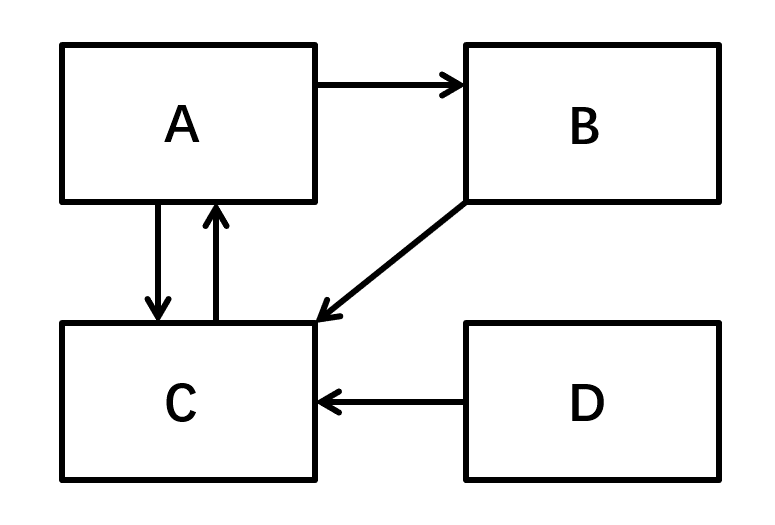
\includegraphics[width=0.6\textwidth]{images/pic1.png}
        \caption{实例1中的简单网络}
    \end{center}
\end{figure}
使用公式(2.1)求出其超链接矩阵
$$
    P=\begin{bmatrix}
        0 & 1/2 & 1/2 & 0 \\
        0 & 0   & 1   & 0 \\
        1 & 0   & 0   & 0 \\
        0 & 0   & 1   & 0
    \end{bmatrix}
$$
取阻尼系数$c=0.85$,计算得到其转移矩阵\
$$
    \widetilde{P}=\begin{bmatrix}
        0.0375 & 0.4625 & 0.4625 & 0.0375 \\
        0.0375 & 0.0375 & 0.8875 & 0.0375 \\
        0.8875 & 0.0375 & 0.0375 & 0.0375 \\
        0.0375 & 0.0375 & 0.8875 & 0.0375 \\
    \end{bmatrix}
$$
其中,$\widetilde{P_{ij}}$表示从页面$i$跳转到页面$j$的概率。

设$t$为迭代次数,当$t=0$时,各网页的PageRank有初始值$0.25$。
$$
    \boldsymbol{x}(0)=\begin{bmatrix}
        0.25 \\0.25\\0.25\\0.25
    \end{bmatrix}
$$
经历第一次迭代后
$$
    \boldsymbol{x}(1)=\begin{bmatrix}
        0.25 \\0.14375\\0.56875\\0.0375
    \end{bmatrix}
$$
可以作图表示从$t=0$到$t=1$时PageRank值的转移情况。
\begin{figure}[H]
    \begin{center}
        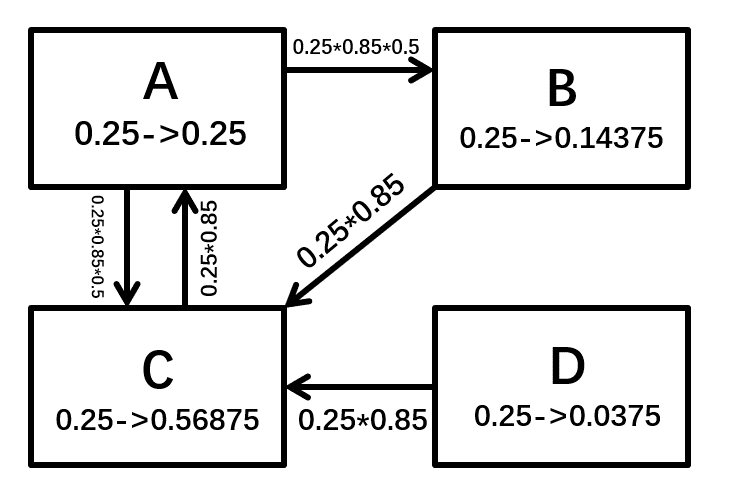
\includegraphics[width=0.65\textwidth]{images/pic1-0-1.png}
        \caption{实例1中从$t=0$到$t=1$时PageRank值的转移情况}
    \end{center}
\end{figure}
可以看出,在每次迭代的过程中,相当于将当前页面的PageRank值乘以阻尼系数$d$,平均地通过超链接转移给目标页面\cite{bi:WX}。

继续进行迭代,待趋于稳定时得到的PageRank值为
$$
    \boldsymbol{\pi}=\begin{bmatrix}
        0.37252685 \\0.19582391\\0.39414924\\0.0375
    \end{bmatrix}
$$
同时也可以作出迭代过程中PageRank值变化的折线图。
\begin{figure}[H]
    \begin{center}
        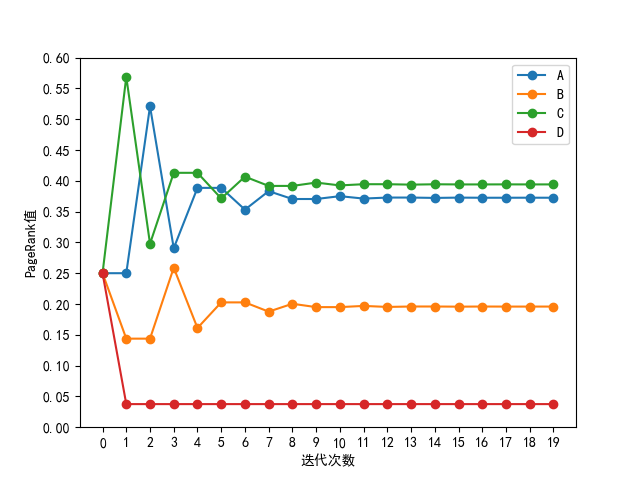
\includegraphics[width=0.80\textwidth]{images/Figure_1.png}
        \caption{实例1迭代过程中PageRank值变化}
    \end{center}
\end{figure}
因此,网页排名的最终结果为$C,A,B,D$。可以发现,网页的PageR ank值与被链接的次数和链接它的界面的PageRank值有关。在这个示例中,页面$C$被链接的次数最多,其PageRank值最高,页面$A,B$被链接的次数相等,但由于链接到$A$的页面$C$的PageRank值更高,即“更优质”,$A$最终的PageRank值高于$B$。而没有页面链接到页面$D$,因此其PageRank值最低。

\section[实例2:阻尼因子$c$的影响]{实例2:阻尼因子$c$的影响}

接下来考虑阻尼因子$c$对PageRank值的影响。

首先,我们考虑与实例1相同的简单网络。
\begin{figure}[H]
    \begin{center}
        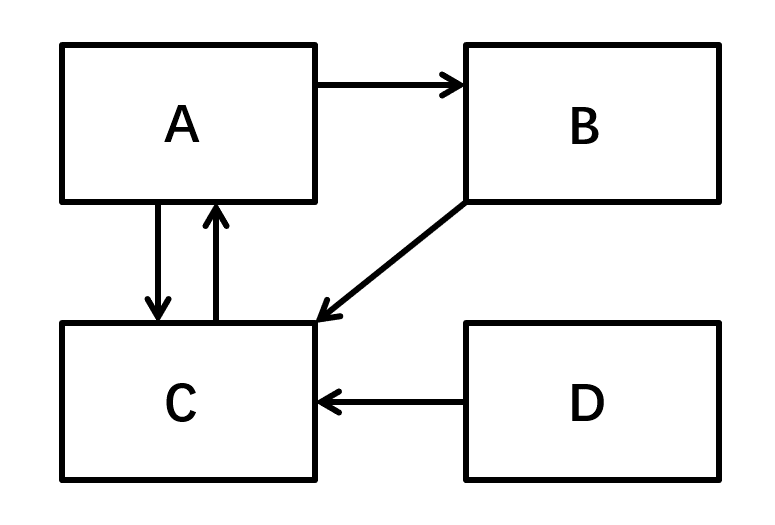
\includegraphics[width=0.6\textwidth]{images/pic1.png}
        \caption{实例2中的简单网络(1)}
    \end{center}
\end{figure}

通过Python程序,我们可以作出各网页的PageRank值随阻尼因子$c$的取值而变化的折线图。

\begin{figure}[H]
    \begin{center}
        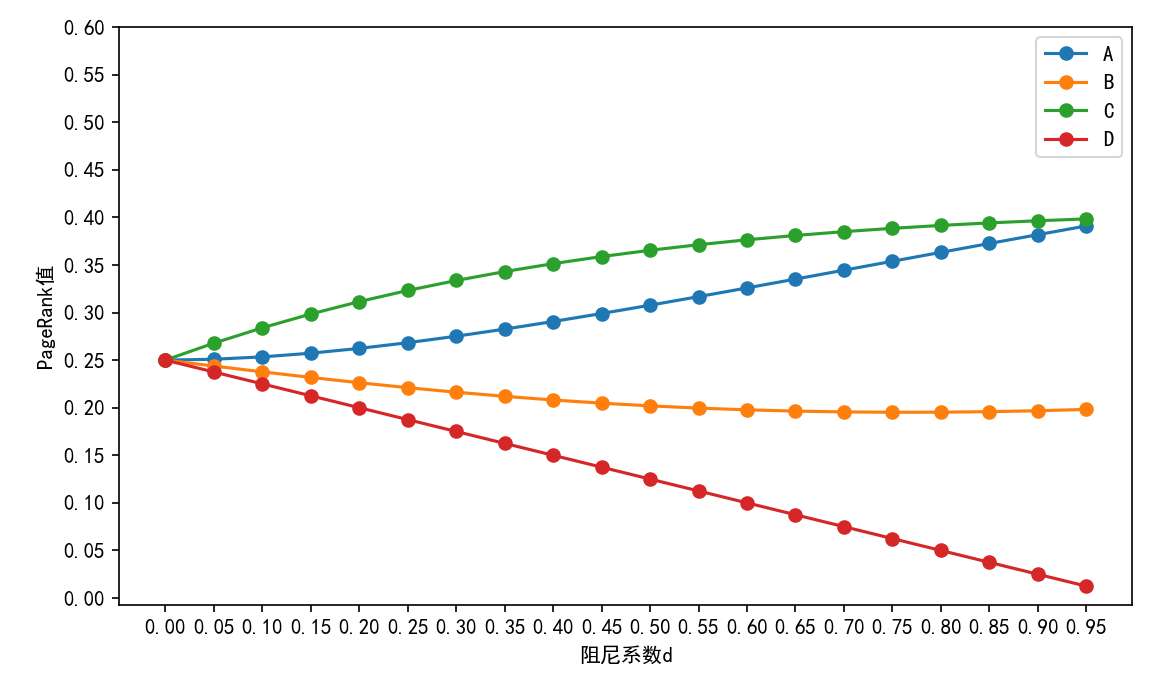
\includegraphics[width=1\textwidth]{images/pic2(1).png}
        \caption{实例2中简单网络(1)中各网页的PageRank值随阻尼因子$c$的变化}
    \end{center}
\end{figure}
可以发现,此时阻尼因子$c$越大,不同网页的PageRank值在大体上差异更大,网页的“优劣”更加容易区分。

接下来,我们考虑一种更简单的网络,如下图所示。
\begin{figure}[H]
    \begin{center}
        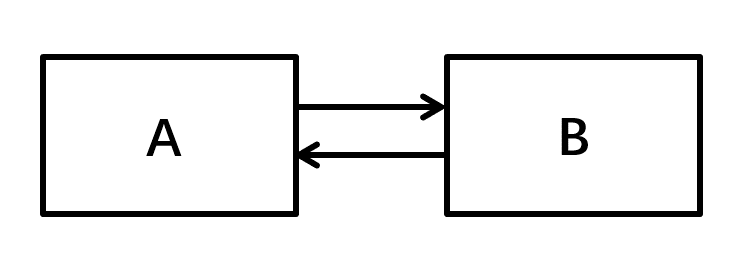
\includegraphics[width=0.6\textwidth]{images/pic2-2.png}
        \caption{实例2中的简单网络(2)}
    \end{center}
\end{figure}

作出其PageRank值随阻尼因子$c$变化的折线图。
\begin{figure}[H]
    \begin{center}
        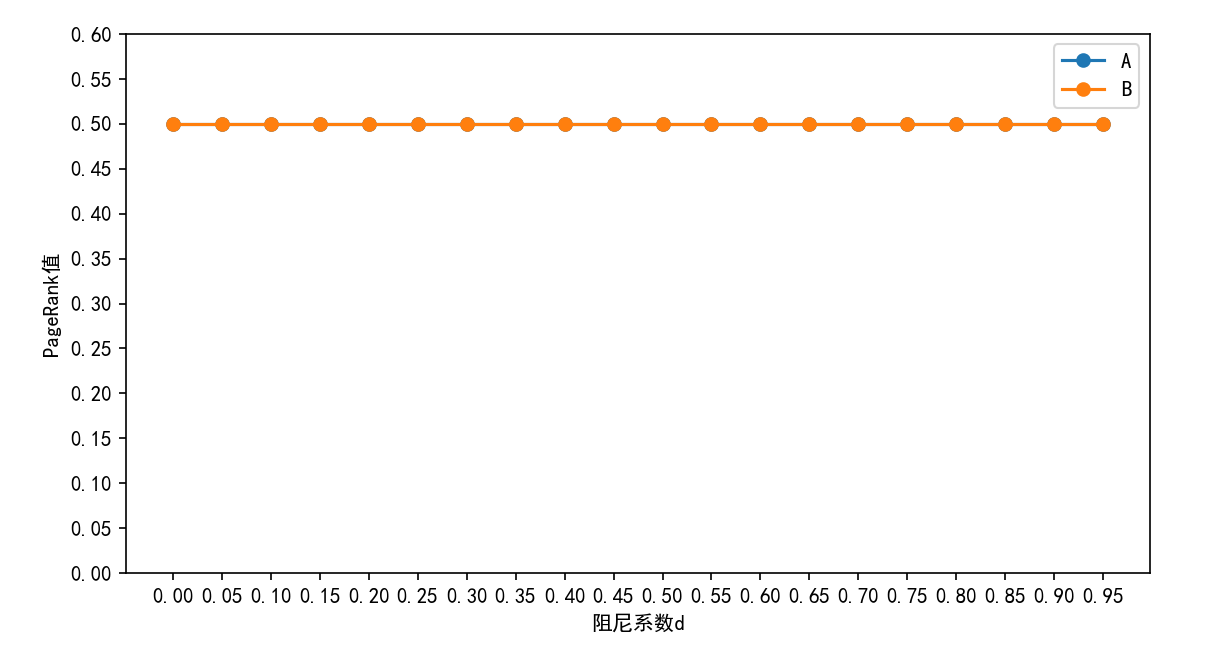
\includegraphics[width=1\textwidth]{images/pic2(2).png}
        \caption{实例2中简单网络(2)中各网页的PageRank值随阻尼因子$c$的变化}
    \end{center}
\end{figure}

不难发现,在这种情况下,其各页面的PageRank值与阻尼因子$c$的取值无关。

接下来,我们考虑另一种样式的简单网络,如下图所示。
\begin{figure}[H]
    \begin{center}
        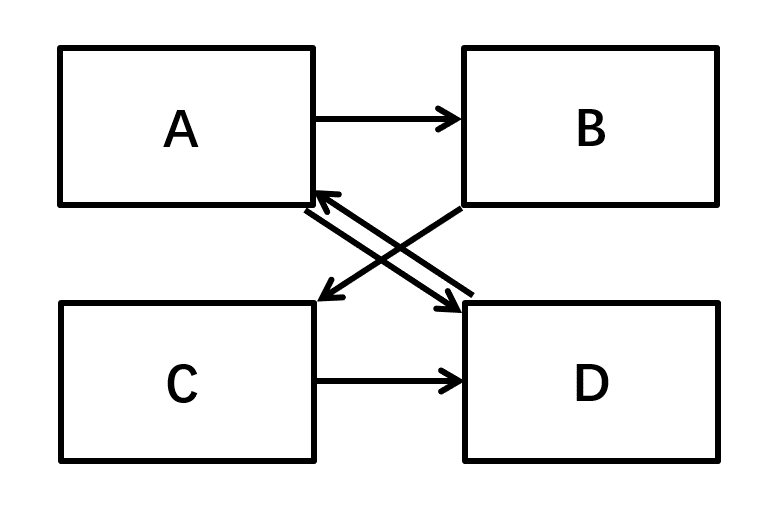
\includegraphics[width=0.6\textwidth]{images/pic2(3).png}
        \caption{实例2中的简单网络(3)}
    \end{center}
\end{figure}

作出其PageRank值随阻尼因子$c$变化的折线图。
\begin{figure}[H]
    \begin{center}
        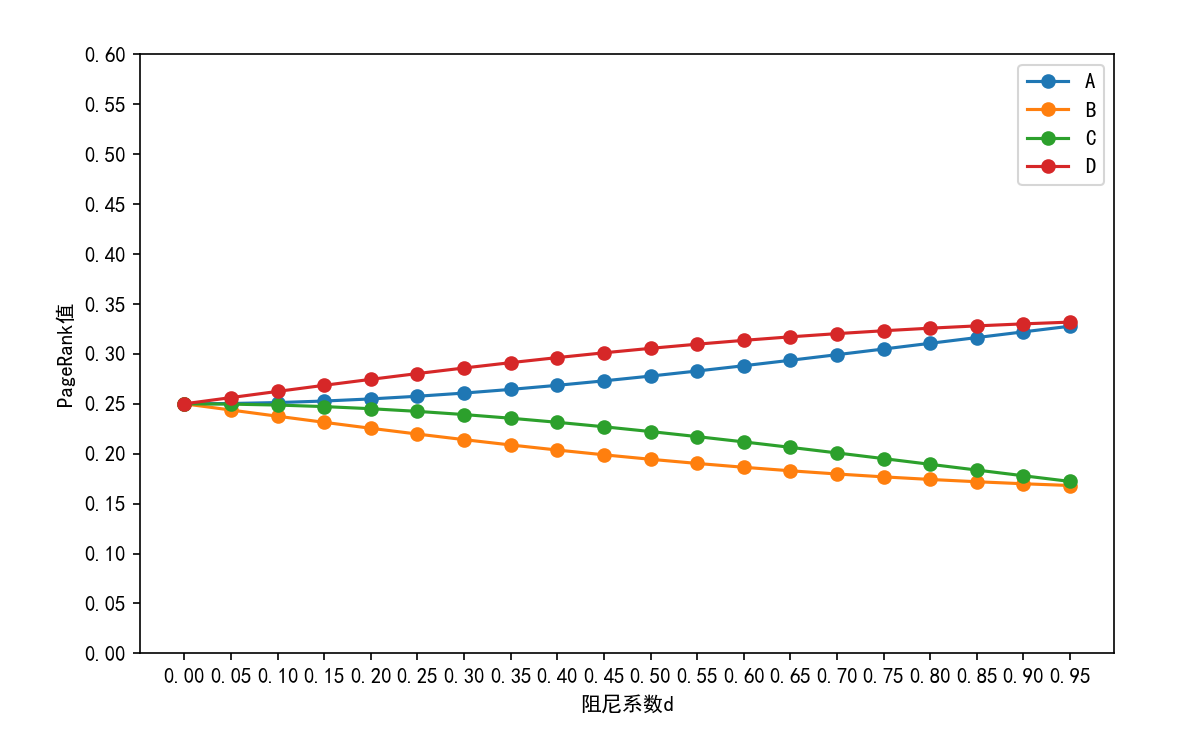
\includegraphics[width=1\textwidth]{images/pic2-3.png}
        \caption{实例2中简单网络(3)中各网页的PageRank值随阻尼因子$c$的变化}
    \end{center}
\end{figure}
可以发现,在这种情况下,阻尼因子$c$取较为靠近中间的值最为合适,过小或过大均会导致网页之间的区分度下降。

根据上述结论,阻尼因子的变动会对不同类型的网络下的不同网页差生影响,具体影响的大小和方式取决于网络的类型。由于马尔可夫链的基本假设与网页搜索的特性相同,经推到得知阻尼因子越接近1效果越好\cite{bi:TW},但在与简单网络(3)类型相似的网络中,阻尼因子太靠近1时,无法区分网页优劣,因此Google取阻尼因子为0.85必有其独特考量\cite{bi:TW,bi:G}。


\chapter[PageRank算法的缺陷与优化]{PageRank算法的缺陷与优化}
\section[缺陷]{缺陷}
虽然 PageRank 算法是一种经典的网页排名算法,但它也有一些缺陷。

其中最明显的缺陷是被称为“均匀访问假设”,即假设用户访问所有网页的概率相等。这并不总是真实情况,因为用户可能更喜欢访问某些网页,例如知名网站和社交媒体网站。

易受到垃圾链接的影响也是一个严重的问题。垃圾链接是指那些存在于低质量网页或通过黑帽SEO手段生成的链接,它们的存在会影响到整个网页排名系统。此外,垃圾链接的使用也可能会导致PageRank算法的误导。例如,一个不相关的网站可以通过将大量的垃圾链接指向某个网站,来提高该网站的排名。例如,Google搜索曾在挪威发生过一次事故,当时,大量搜索结果被某名为垃圾网站占据(“美人鱼事件”)。攻击者可以通过构建大量的虚假网页,并将这些网页与目标网站进行链接,从而提高目标网站的排名。为了应对这种风险,Google等搜索引擎采用了各种反作弊措施,例如对网页质量进行评估、监控垃圾链接等。

另一个PageRank算法的缺陷是难以处理动态网页。如果一个网页的内容经常变化,PageRank算法可能无法及时反映这些变化。例如,一些新闻网站每天都会发布大量新闻,如果PageRank算法只在网站更新时计算一次,那么这些新闻的重要性将无法及时反映到排名中。为了解决这个问题,一些搜索引擎采用了实时计算PageRank的方法。

PageRank算法还存在数据稀疏性和主题缺乏的问题。在某些情况下,由于缺乏与搜索主题相关的网页链接,PageRank算法可能会忽略一些重要的网页。此外,由于PageRank算法只考虑链接结构,而忽略网页的内容和主题,因此它可能无法很好地适应某些特定领域的搜索,例如医疗、法律等领域。



\section[优化]{优化}
\subsection[矩阵分解的应用]{矩阵分解的应用}
在互联网上,网页的数量极为庞大,因此如何高效地计算网页的PageRank值成为了一个关键问题。为了跟上互联网结构的迅速变化,Google每月更新一次PageRank。其中一种方法便是探索超链接矩阵$P$的特定性质\cite{bi:DGPOLS}。在本部分中,我们将利用矩阵$P$的可约性来进行优化。

考虑如下形式的超链接矩阵$P$
\begin{equation}
    P=\begin{bmatrix}
        P_1    & \cdots & 0      \\
        \vdots & \ddots & \vdots \\
        0      & \cdots & P_N    \\
    \end{bmatrix}
\end{equation}
其中,对角线上的块$P_I(I=1,\dots,N)$表示第$I$组内的链接。我们用$n_I$来表示第$I$组内部的网页个数。每个块$I$不与外界交流,但其本身内部可能存在着非常复杂的关系。

接下来,我们考虑超链接矩阵(4.1)所对应的转移矩阵$\widetilde{P}=cP+(1-c)(1/n)E$,令向量$\boldsymbol{\pi}$为转移矩阵$\widetilde{P}$的PageRank向量,其满足$\boldsymbol{\pi} \widetilde{P}=\boldsymbol{\pi},\boldsymbol{\pi}\boldsymbol{e}=1$。此外,我们定义块$I$的摄动矩阵
\begin{equation}
    \widetilde{P_I}=cP_I+\frac{1-c}{n_I}E
\end{equation}
并令向量$\boldsymbol{\pi}_I$为$\widetilde{P_I}$的PageRank向量,使得
\begin{equation}
    \boldsymbol{\pi}_I \widetilde{P_I}=\boldsymbol{\pi}_I,\quad\boldsymbol{\pi}_I\boldsymbol{e}=1
\end{equation}

可以证明得到以下公式

\begin{equation}
    \boldsymbol{\pi}=\frac{1}{n}\left(n_1\boldsymbol{\pi_1},n_2\boldsymbol{\pi_2},\dots,n_N\boldsymbol{\pi_N}\right)
\end{equation}
\textbf{证明}

我们可以证明(4.4)确实为$\widetilde{P}$的平稳分布。定义
\begin{equation}
    \overline{E}=\begin{bmatrix}
        \frac{1}{n_1}E & \cdots & 0              \\
        \vdots         & \ddots & \vdots         \\
        0              & \cdots & \frac{1}{n_N}E \\
    \end{bmatrix}
\end{equation}
对于式(4.4)中的$\boldsymbol{\pi}$,有
\begin{equation}
    \begin{aligned}
        \boldsymbol{\pi}\widetilde{P}
         & = \boldsymbol{\pi}\left[cP+(1-c)\overline{E}-(1-c)\overline{E}+(1-c)(1/n)E\right]                                                                                            \\
         & = \boldsymbol{\pi}\left[cP+(1-c)\overline{E}\right]+\boldsymbol{\pi}\left[(1-c)(1/n)E-(1-c)\overline{E}\right]                                                               \\
         & = \left(\frac{n_1}{n}\boldsymbol{\pi_1}\widetilde{P_1},\dots,\frac{n_N}{n}\boldsymbol{\pi_N}\widetilde{P_N}\right)+(1-c)(1/n)\boldsymbol{e}^{T}-(1-c)(1/n)\boldsymbol{e}^{T} \\
         & = \frac{1}{n}\left(n_1\boldsymbol{\pi_1},n_2\boldsymbol{\pi_2},\dots,n_N\boldsymbol{\pi_N}\right)                                                                            \\
         & = \boldsymbol{\pi}
    \end{aligned}
\end{equation}
由于$\widetilde{P}$的PageRank向量是唯一的,因此$\boldsymbol{\pi}$即为$\widetilde{P}$的PageRank向量。

该定理的证明是较为容易的。这种分解特性也可以用以下公式来表示
\begin{equation}
    \boldsymbol{\pi}=\frac{1-c}{n}\boldsymbol{e}^{T}\left[1-cP\right]^{-1}
\end{equation}

接下来让我们讨论该公式对PageRank结果计算的意义。如果我们预先不知道超链接矩阵的块结构,则可以使用任何的图遍历算法来得到(如深度优先搜索算法和广度优先搜索算法)。图遍历算法的时间复杂度为$O(n + m)$,其中$n$为网页的数量,$m$为链接的数量。但是注意到超链接矩阵是极其稀疏的,时间复杂度在页面数量上接近线性。由于我们对超链接矩阵进行了分解,可以独立地处理所分成的每一个部分并将PageRank近似向量的不同部分存储在不同的数据库中,来达到节省时间和空间的目的。特别的,我们可以考虑使用尽可能多的并行处理器来进行运算,从而得到更好的计算效率。


\subsection[主题敏感的PageRank算法]{主题敏感的PageRank算法}

主题敏感的PageRank算法(Topic-sensitive PageRank)是PageRank算法的一种扩展,旨在提高搜索结果的准确性。与传统的PageRank算法不同,它不再只考虑页面的全局重要性,而是基于给定主题的重要性对页面进行排序。这种算法对于需要特定主题的搜索结果更为有效。

Topic-sensitive PageRank的主要思想是根据预定义的主题构建多个PageRank向量,每个向量都有自己的主题,并使用它们来计算页面的权重。在常规关键字搜索查询中,可以使用查询关键字的主题计算页面的主题敏感PageRank分数。而在上下文搜索中(例如,当在网页中选中一些文字进行搜索查询时),可以使用查询出现的上下文的主题来计算页面的主题敏感PageRank分数。通过使用这些(预先计算好的)主题偏置PageRank向量的线性组合,可以在查询时生成特定上下文下的页面重要性分数,从而比使用单个通用PageRank向量生成更准确的排名结果。\cite{bi:TC}

\begin{figure}[H]
    \begin{center}
        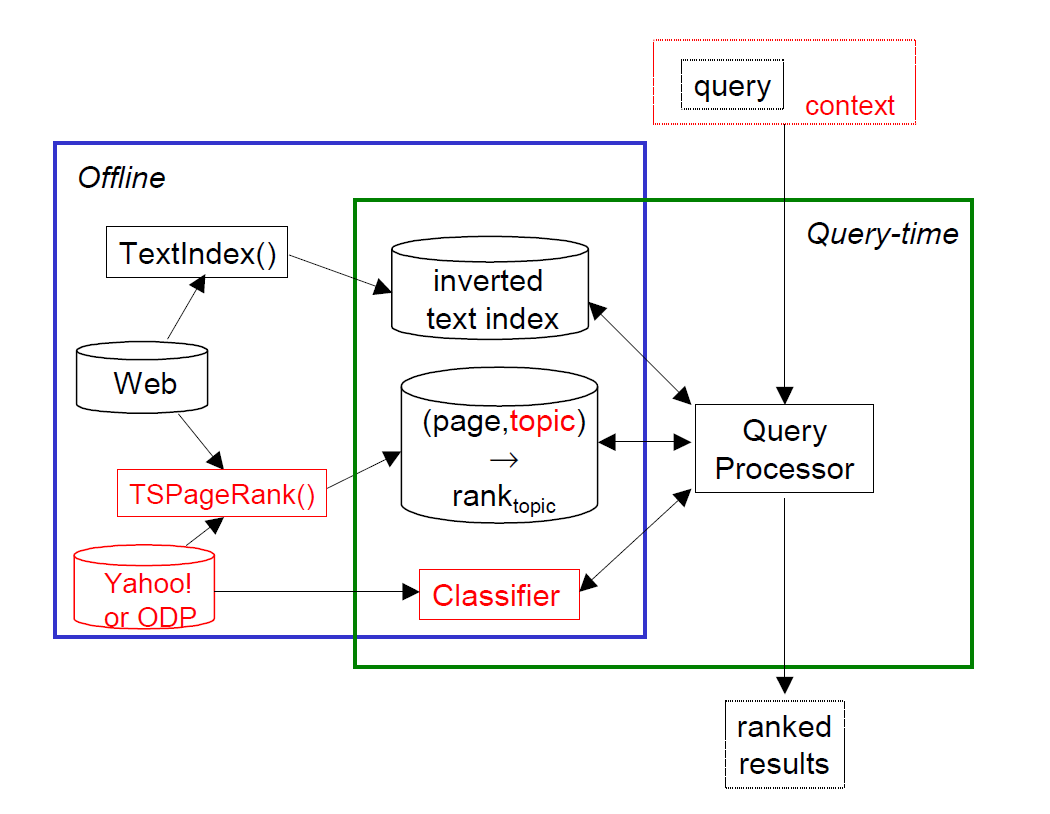
\includegraphics[width=0.9\textwidth]{./images/topic_sensitive.png}
        \caption{使用主题敏感的PageRank的系统示意图\cite{bi:TC}}
    \end{center}
\end{figure}

此方法的概述如下\cite{bi:TC}。在离线处理Web爬虫期间,我们使用Open Directory Project (ODP,一份包含超过250万个URL的Web目录)中的顶级类别的URL生成16个主题敏感的PageRank向量。在查询时,我们计算查询(或用户上下文)与每个主题的相似度。然后,我们不使用单个全局排名向量,而是使用主题敏感向量的线性组合,加权使用查询(和任何可用上下文)与主题之间的相似度。通过使用一组排名向量,我们能够更准确地确定与特定查询或查询上下文相关的最重要的页面。由于基于链接的计算在预处理阶段进行离线处理,因此查询时间成本不比普通PageRank算法高。

\subsection[稀疏矩阵优化]{稀疏矩阵优化}

PageRank算法中,最消耗计算资源的部分就是计算网页之间的链接权重,这涉及到对每个网页的出链进行求和。由于大多数网页的出链数量非常庞大,因此这个过程会产生一个非常稀疏的矩阵。为了有效地处理这个问题,可以使用稀疏矩阵优化技术。

在PageRank算法中,每个网页可以表示为一个节点,每个链接可以表示为从一个节点到另一个节点的边。我们可以将这些节点和边表示为一个稀疏矩阵,其中矩阵中的每个元素表示一个链接的权重。
在传统的矩阵计算中,我们需要处理整个矩阵,即使其中大部分元素是0。然而,在PageRank算法中,矩阵非常稀疏,因此可以使用稀疏矩阵优化技术,只处理非零元素,从而减少计算量。

稀疏矩阵优化的一种方法是使用压缩稀疏行(Compressed Sparse Row,CSR)格式。在CSR格式中,矩阵中的每个非零元素都保存了其值、列索引和行偏移量。行偏移量指示了每一行中第一个非零元素的位置,这使得矩阵的每一行都可以通过一个单独的数组来表示。

这种方法可以大大降低计算复杂度,因为只需要处理非零元素。在PageRank算法中,使用CSR格式可以减少计算时间和内存消耗,从而使算法可以处理更大的网页集合\cite{bi:ACM}。

\chapter[PageRank算法在人工智能中的应用]{PageRank算法在人工智能中的应用}
\thispagestyle{fancy}

PageRank算法最初是为了互联网搜索引擎的排序问题而提出的,但是随着人工智能的不断发展,PageRank算法也被应用到了更多的领域。在本章节,我们将简要介绍PageRank算法在人工智能中可能的(或已经存在的)应用。

\section[自然语言处理]{自然语言处理}

PageRank算法在自然语言处理中的应用比较广泛,其中一种应用是关键词提取。
关键词抽取是一种自然语言处理任务,旨在从文本中提取最具代表性的关键词或短语。PageRank算法可以用于对文本中的关键词进行排序,以确定最具有代表性的关键词。该方法使用单词之间的相似性和共现关系构建词语网络,并利用PageRank算法确定在该网络中最重要的单词。例如,可以基于PageRank算法,并结合人类语言习惯特性定义位置权重系数,实现新闻关键词提取算法\cite{bi:XW}。

PageRank算法还可用于文本分类任务,其中目标是将文本分为不同的类别。在这种情况下,每个类别可以视为单词网络中的一个节点。利用PageRank算法可以计算每个节点的权重,以便更好地理解哪些节点在文本分类中是最重要的。例如,借鉴于PageRank模型和跨领域倾向性
分析算法,通过引入PageRank模型来研究词汇的原始情感倾向性识别技术,来判断情感词表现出的情感极性\cite{bi:QG}。

\section[聊天机器人]{聊天机器人}

近期,Chat GPT的大热让我们关注于聊天机器人和大模型。可以考虑将PageRank(实际上即为搜索引擎)与聊天机器人相结合,以提高其智能程度。当结合PageRank算法和聊天机器人时,可以将聊天机器人看作是一个搜索引擎的前端。与传统的搜索引擎不同,聊天机器人可以提供更加个性化和交互式的搜索结果,从而更好地满足用户的需求。

例如,当用户输入一个问题或者话题时,聊天机器人可以使用PageRank算法对相关网页进行排名,并展示给用户最有用的信息。这样,聊天机器人就可以像一个个性化的搜索引擎一样,为用户提供最相关和有用的答案。而且,通过分析用户与网页的交互行为,聊天机器人可以不断学习和优化PageRank算法的权重和参数,提高其预测和推荐的准确性。另外,聊天机器人还可以使用PageRank算法来帮助用户发现与他们感兴趣的主题相关的内容。例如,当用户询问聊天机器人有关特定主题的信息时,聊天机器人可以使用PageRank算法来推荐与该主题相关的最佳文章或网页。

然而,目前我们无法确定结合了搜索引擎的聊天机器人Bing AI是否使用PageRank算法。不过,我们仍然可以对这个方向进行展望,结合PageRank和聊天机器人仍然是一个有潜力的领域。

\chapter[启发和体会]{启发和体会}
\thispagestyle{fancy}

在调研和分析PageRank算法的过程中,我们深刻体会到了数学思维的重要性。在平时,我们总是会把数学思维抽象化,认为这是一种虚无缥缈的,难以捉摸的东西。但是在PageRank的研究中,我们却能够切身的体会到数学思维对我们实际的应用。矩阵的向量运算,矩阵的特征向量和特征值,这些我们平时只会把其当作“烦人”的题目。而在人工智能领域中,这却能搭建出整个具体项目的框架。

首先, PageRank算法的核心思想是基于矩阵运算的。在PageRank算法中,链接关系可以被看作一张有向网图,网页之间的链接关系可以被表示为一个转移矩阵。在这个矩阵中,每个网页都对应其中的一行或一列,矩阵某一位置的值表示从该网页到另一个网页的链接权重。利用矩阵乘法运算,可以简单地计算每个网页之间的链接值,并将其转化为一种线性代数问题。将本身宏观的现象处理为一种具体的可操作的问题,这就是数学的伟大之处吧。就像我们在学计算机之前,很难去想象我们手上的这台机器实际上是在处理一堆数据。

其次, PageRank算法基于马尔科夫链模型进行设计。马尔科夫链模型是一种随机过程,通过描述状态之间的转移发生,可以用于计算一些存在随机性和时序性变化的系统的属性。PageRank算法中将每个网页看作马尔科夫链中的一个状态,网页间的链接关系看作状态之间的转移关系。根据网页之间链接的质量和数量不同,不同状态之间转移的概率不同,使得PageRank算法能够通过迭代计算贡献率,动态调整不同网页之间PageRank值的权重和排名。将这些抽象化的数据,链接在一起,形成联系,最后总结出一个能写出来的公式,这也是数学的神奇之处。事实上,

在各项研究之中,数学几乎都可以展现它魅力,就例如,学习与记忆这种抽象的事物,研究者也能通过这总结出规律,称之为艾宾浩斯遗忘曲线(The Ebbinghaus Forgetting Curve)。要知道这条规律被总结出来的时候是1885年,人们收集数据,总结分析的能力,是远远不如今天的,更何况,人工智能的出现更是大大加快了速率,所以数学的规律必将在今日今时得到飞跃性的体现。

最后,PageRank算法也是一种基于迭代的算法为了计算每个网页的PageRank值,PageRank算法需要进行多轮迭代计算。在迭代的过程中,每个网页的贡献率和PageRank值都会被不断修正和更新,直到达到稳定状态。此时,计算得到的PageRank值就是最终的结果。要知道,迭代运算在计算机处理问题中是一种必不可少的方法,它能找到一个无解的问题无限接近实际的最优解,就比方说,谷歌搜索时的相关性,本身是一个因人而异的东西的,而PageRank利用迭代,却能找出一个所有人几乎都认可的结果。

此外在研究过程中,我们也联想到了一些现实的问题。例如,在社交网络中,PageRank算法可以通过计算用户之间的关联度评估用户的影响力和网络地位;在生物信息学中,PageRank算法可以被用来构建蛋白质相互作用网络。这些应用反映出PageRank算法的高度可扩展性,并突出了算法本身的优越性。同时,我们也想到在强大的算法背后引申出来的一些问题。随着全球化的发展,互联网已经成为企业和政府在国际市场上竞争的重要手段之一。然而,互联网上的信息量巨大,用户容易受到信息过载和信息误导的困扰。在这种情况下,PageRank算法的应用可以在一定程度上解决这个问题。对于在互联网上进行品牌推广和营销的企业来说,提高网站的PageRank分数可以增加网站的搜索引擎排名,从而增加网站的曝光率,并吸引更多的潜在客户。在这种优势的背后如果有人从中作恶,故意误导风向,那后果可想而知。我想往后人工智能也需解决这类问题。

总之,PageRank算法是一种基于数学思维的,能用于具体程序的,具有优越性的算法。研究它都使我们对于人工智能的数学思维理解的更加深刻。

\newpage
\setlength{\bibsep}{1ex}  % 需 natbib 宏包
\begin{thebibliography}{99}
    \addcontentsline{toc}{chapter}{参考文献}
    \thispagestyle{fancy}

    % \addtolength{\itemsep}{-5pt}

    \bibitem{bi:SG}
    Search Engine Market Share Worldwide, Statcounter GlobalStats, 2023, \url{https://gs.statcounter.com/search-engine-market-share}

    \bibitem{bi:G}
    Brin, S., Page, L.. The anatomy of a large-scale hypertextual Web search engine. Computer Networks and ISDN Systems.,1998, 30(1–7): 107–117.

    \bibitem{bi:RA}
    Rajeev Motwani, Prabhakar Raghavan. Randomized Algorithms. Cambridge University Press, United Kingdom, 1995.

    \bibitem{bi:DGPOLS}
    Avrachenkov K, Litvak N. Decomposition of the google pagerank and optimal linking strategy[D]. INRIA, 2004.

    \bibitem{bi:WX}
    吴淑燕, 许涛. PageRank 算法的原理简介[J]. 图书情报工作, 2003, 47(2): 55.

    \bibitem{bi:TW}
    傅懷慧, 林共進, 白峰杉, 等. 阻尼因子對網頁排名之敏感度分析[J]. 中國統計學報, 2005, 43(2): 145-164.

    \bibitem{bi:TC}
    Haveliwala T H. Topic-sensitive pagerank[C]. Proceedings of the 11th international conference on World Wide Web. 2002: 517-526.

    \bibitem{bi:ACM}
    Gruetzmacher, T.; Cojean, T.; Flegar, G.; Anzt, H.; Quintana-Orti, ES. (2020). Acceleration
    of PageRank with customized precision based on mantissa segmentation. ACM
    Transactions on Parallel Computing. 7(1):1-19. \url{https://doi.org/10.1145/3380934}

    \bibitem{bi:XW}
    顾亦然,许梦馨.基于PageRank的新闻关键词提取算法[J].电子科技大学学报,2017(5):777-783.

    \bibitem{bi:QG}
    李荣军, 王小捷, 周延泉. PageRank 模型在中文情感词极性判别中的应用[J]. 北京邮电大学学报, 2010, 33(5): 141.

\end{thebibliography}

\newpage
\addcontentsline{toc}{chapter}{附\quad 录}
\begin{center}
    \vspace{-3.5em}\centerline{\zihao{-3}\textbf{\heiti 附\quad 录}}\vspace{-0.7em}
\end{center}
% \begin{tabular}{p{0cm}p{5.5em}@{\extracolsep{0.5ex}}p{0cm}p{0em}cc}
%     ~ & \hfill 贡 \quad 献: &  & \mcc{李鹏达 10225101460 } &  & \mcc{$25\%$} \\
%     ~ & \hfill               &  & \mcc{武泽恺 10225101429 }  &  & \mcc{$25\%$} \\
%     ~ & \hfill               &  & \mcc{吴泽霖 10225101428 }  &  & \mcc{$25\%$} \\
%     ~ & \hfill               &  & \mcc{张耘彪 10225101437 }  &  & \mcc{$25\%$} \\
% \end{tabular}
\linespread{1.4}
\begin{table}[H]
    \centering
    \begin{tabular}{p{3cm}p{3.3cm}p{0.1cm}p{0.7cm}}
      \textbf{\heiti \zihao{-4} 小组成员贡献:} & \heiti  李鹏达 10225101460 & \, & $\bold{25}\%$            \\ \cline{2-2} \cline{4-4}
      & \heiti  武泽恺 10225101429 & \, & $\bold{25\%}$            \\ \cline{2-2} \cline{4-4}
      & \heiti  吴泽霖 10225101428 & \, & $\bold{25}\%$            \\ \cline{2-2} \cline{4-4}
      & \heiti  张耘彪 10225101437 & \, & $\bold{25}\%$            \\ \cline{2-2} \cline{4-4}
    \end{tabular}
  \end{table}
\end{document}